\documentclass[final]{beamer}
\mode<presentation>{\usetheme{Lankton}}
\usepackage{verbments}
%\usepackage{amsmath,amsfonts,amssymb,pxfonts,eulervm,xspace}
\usepackage{amsmath,amsfonts,amssymb}
%pxfonts,eulervm,xspace}
\usepackage{graphicx}
\usepackage{color}
\usepackage[orientation=landscape,size=custom,width=101,height=76,scale=2.3,debug]{beamerposter}

\usepackage{wrapfig}

\usepackage[export]{adjustbox}

\usepackage{tikz}
\usetikzlibrary{calc,trees,positioning,arrows,chains,shapes.geometric,%
    decorations.pathreplacing,decorations.pathmorphing,shapes,%
    matrix,shapes.symbols}

\tikzset{
>=stealth',
  pointchain/.style={
    rectangle, 
    rounded corners, 
    % fill=black!10,
    draw=black, very thick,
    text width=10em, 
    minimum height=3em, 
    text centered, 
    on chain},
  line/.style={draw, thick, <-},
  element/.style={
    tape,
    top color=white,
    bottom color=blue!50!black!60!,
    minimum width=8em,
    draw=blue!40!black!90, very thick,
    text width=10em, 
    minimum height=3.5em, 
    text centered, 
    on chain},
  every join/.style={->, thick,shorten >=1pt},
  decoration={brace},
  tuborg/.style={decorate},
  tubnode/.style={midway, right=2pt},
}


\usebackgroundtemplate%
{%
%    \includegraphics[width=\paperwidth,height=\paperheight]{blackness.png}%
}


%-- Header and footer information ----------------------------------
\newcommand{\footleft}{\texttt{https://curatedcourses.org/}}
\newcommand{\footright}{\scriptsize\parbox{21in}{\raggedleft\color{gray} CuratedCourses is based upon work supported
  by the National Science Foundation under NSF DUE--1505246.\\ Any
  opinions, findings, and conclusions or recommendations expressed in
  this material are those of the author(s) and do not necessarily
  reflect the views of the National Science Foundation.}
\raisebox{-1in}{\includegraphics[width=3in]{qrcode.pdf}}}
\title{Supported by NSF Grant NSF DUE--1505246}
\author{Petra Bonfert-Taylor, Sarah Eichhorn, David Farmer, Jim Fowler}
%-------------------------------------------------------------------


%-- Main Document --------------------------------------------------
\begin{document}
{

\newenvironment{sectionblock}[1]{\begin{block}{\rule{0pt}{1in}#1}}{\end{block}}

%\usebackgroundtemplate{\includegraphics[height=\paperheight]{blackness.png}}
\begin{frame}[fragile]{}
  \begin{columns}[t]

    %-- Column 1 ---------------------------------------------------
    \begin{column}{0.32\linewidth}
      % -- Block 1-1
\begin{sectionblock}{THIS}
So much content!
\end{sectionblock}

\begin{block}{\rule{0pt}{1in}Begin with \LaTeX}
  \tiny
\end{block}




    \end{column}%1

    %-- Column 2 ---------------------------------------------------
    \begin{column}{0.32\linewidth}
            %-- Block 2-1
      \begin{block}{\rule{0pt}{1in}Serve Online}
        \begin{figure}[htb]
          \centering
          %\includegraphics[width=.9\columnwidth]{ximeraMoon}
        \end{figure}
      \end{block}

      \begin{block}{\rule{0pt}{1in}\raisebox{.2\height}{Fight Bit Rot}}
\footnotesize 
\LaTeX\ was first released in 1984.\\
\LaTeXe\ was released in 1994. \\
Longevity is key to preserving an author's work.
      \end{block}


    \end{column}%2

    %-- Column 3 ---------------------------------------------------
    \begin{column}{0.32\linewidth}
      \begin{sectionblock}{Multiple Textbooks}

  Tagging an open-source linear algebra textbook with the
  CuratedCourses taxonomy enables the margin of the textbook to be populated with relevant open
  resources.\\[1ex]

  And not only can resources be aligned to textbooks, but the textbooks can also be aligned with each other.

  \begin{figure}
    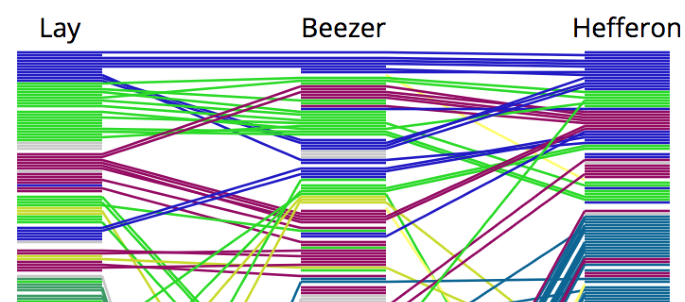
\includegraphics[width=0.9\textwidth]{alignment.pdf}
  \end{figure}


\end{sectionblock}



\begin{sectionblock}{Workshop and Minicourse}
  As part of the project, the team runs workshops to train
  faculty in the development of and the use of open content, including
  a minicourse at the Joint Math Meetings in January 2018 and a
   workshop in August 2018.


\end{sectionblock}



    \end{column}
 
  \end{columns}
\end{frame}
}
\end{document}
